\documentclass{article}
\usepackage{amssymb}
\usepackage{amsmath}
\usepackage{mathtools}
\usepackage{cancel}
\usepackage{tikz}
\usepackage{hyperref}
\usepackage{circuitikz}
\usepackage{float}
\usepackage{afterpage}
\usepackage{pgfplots}
\usepackage{textcomp}
\usepgfplotslibrary{groupplots}
\usetikzlibrary{calc, arrows}
\newtheorem{theorem}{Theorem}
\newtheorem{definition}{Definition}
\newtheorem{corollary}{Corollary}
\newtheorem{proof}{Proof}
\tikzstyle{int}=[draw, fill=blue!20, minimum size=2em]
\tikzstyle{init} = [pin edge={to-,thin,black}]

\tikzstyle{block} = [draw, fill=blue!20, rectangle, 
    minimum height=3em, minimum width=6em]
\tikzstyle{sum} = [draw, fill=blue!20, circle, node distance=1cm]
\tikzstyle{input} = [coordinate]
\tikzstyle{output} = [coordinate]
\tikzstyle{pinstyle} = [pin edge={to-,thin,black}]

\DeclareMathOperator*{\argmin}{argmin}

\begin{document}
\title{EE123 Course Notes}
\author{Anmol Parande}
\date{Spring 2020 - Professor Miki Lustig}
\maketitle
\textbf{Disclaimer: }These notes reflect EE123 when I took the course (Spring 2020). They may not accurately reflect current course content, so use at your own risk.
If you find any typos, errors, etc, please raise an issue on the \href{https://github.com/parandea17/BerkeleyNotes}{GitHub repository}.\\
\tableofcontents
\newpage
\section{The DFT}
Whereas the CTFT takes a continuous signal and outputs a continuous frequency spectrum and the DTFT takes a discrete signal
and outputs a continuous, periodic frequecy spectrum, the Discrete Fourier Transform takes a discrete finite signal and outputs
a discrete frequency spectrum. This is useful for signal processing because we cannot store infinite signals in a computers memory.
\begin{definition}
    For a length $N$ finite sequence $\{x[n]\}^{n-1}_{0}$, the Discrete Fourier Transform of the signal
    is a length N finite sequence $\{X[k]\}^{n-1}_{0}$ where
    $$X[k] = \sum_{n=0}^{N-1}{x[n]e^{-j\frac{2\pi}{N}kn}}$$
\end{definition}
One way to interpret the DFT is in terms of the Fourier series for a disrete periodic signal $\tilde{x}[n]=x[((n))_N]$. Recall that the coefficient of the kth term of the Fourier Series is
$$a_k = \frac{1}{N}\sum_{n=0}^{N-1}{x[n]e^{-j\frac{2\pi}{N}kn}}$$
Notice that the $a_k$ of the Fourier Series are the DFT values except scaled by a factor of $N$. This gives an intuitive inverse DFT.
\begin{definition}
    For a length N finite sequence $\{X[k]\}^{N-1}_{0}$ representing the DFT of a finite perioidc signal $\{x[n]\}^{N-1}_{0}$,
    the inverse DFT is given by
    $$x[n] = \frac{1}{N}\sum_{k=0}^{N-1}{X[k]e^{j\frac{2\pi}{N}kn}}$$
\end{definition}
Notice that the DFT and the IDFT are very similar in form. It turns out that the IDFT can be expressed as a DFT of $X^*[k]$. Namely
$$IDFT\{X[k]\} = \frac{1}{N}DFT\{X^\star[k]\}^\star$$
Further intuition for the DFT comes from relating it to the DTFT. Suppose we have a finite signal $x[n]$ which is $0$ for $n < 0$ and $n > N-1$.
The DTFT of this signal is
$$X(\omega) = \sum_{n=-\infty}^{\infty}{x[n]e^{-j\omega n}} = \sum_{n=0}^{N-1}{x[n]e^{-j\omega n}}$$
Suppose we sample the DTFT at intervals of $\frac{2\pi}{N}k$, then
$$X[k] = X\left(\frac{2\pi}{N}k\right) = \sum_{n=0}^{N-1}{x[n]e^{-j\frac{2\pi}{N}k n}}$$
Thus we can think of the DFT as a $N$ point sample of the DTFT.
One important point to notice though is that while the DTFT is often centered around 0, because we are summing
from 0 to N-1 in the DFT, the DFT coefficients are centered around $\pi$.
\subsection{Convolution and the DFT}
\subsubsection{Circular Convolution}
When the DFT coefficients of two signals are multiplied, the resulting coefficients describe a circular convolution of the original two signals.
$$x[n]\circledast y[n] \leftrightarrow X[k]Y[k]$$
The circular convolution is defined as follows
$$x[n]\circledast y[n] = \sum_{m=0}^{N-1}x[m]y[((n-m))_N]$$
The mechanics of the circular convolution are the same as that of the regular convolution, except the signal is circularly shifted.
\begin{figure}[h!]
  \centering
  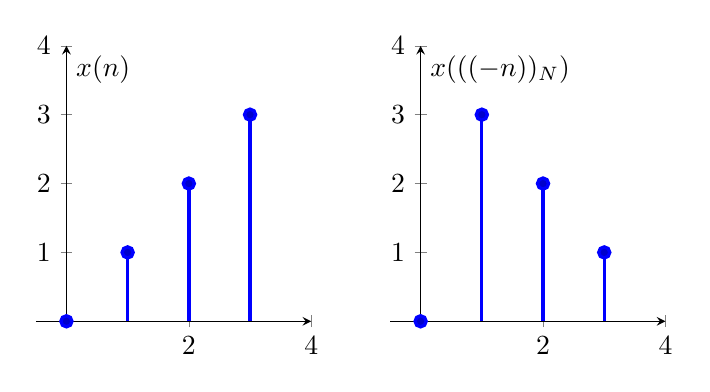
\begin{tikzpicture}
    \begin{groupplot}[
        group style={group size=2 by 1},
        axis lines=middle,
        width=2in,
        height=2in,
        ymax=4]
      \nextgroupplot[ylabel=$x(n)$, xmin=-0.5, xmax=4];
      \addplot+[ycomb, line width=1.2pt] plot coordinates {(0, 0) (1, 1) (2, 2) (3, 3)};
      \nextgroupplot[ylabel=$x(((-n))_N)$, xmin=-0.5, xmax=4];
      \addplot+[ycomb, line width=1.2pt] plot coordinates {(0, 0) (1, 3) (2, 2) (3, 1)};
    \end{groupplot}
  \end{tikzpicture}
  \caption{A circular shift}
\end{figure}
A circular convolution is equivalent to a periodic convolution over a single period.
\subsubsection{Linear Convolution with the DFT}
Because multiplying DFT coefficients performs a convolution, it turns out that we can compute a linear convolution using the circular convolution.
\begin{align*}
  x[n] \qquad 0\le n\le L-1\\
  h[n] \qquad 0 \le n \le P-1
\end{align*}
The linear convolution of these two signals will be length $L+P-1$, so in order to take an IDFT and get $L+P-1$ samples, we need to
take at least $N\le L+P-1$ points.
\begin{itemize}
  \item[1.] Pad each vector to length $L+P-1$
  \item[2.] Compute $X[k]H[k]$
  \item[3.] Take the Inverse DFT
\end{itemize}
If $N$ is too small, the result is akin to aliasing in the time domain.
To see why, consider that the DFT coefficients are essentially the DFS coefficients of the periodic extension of $x[n]$
$$\tilde{x}[n]=\sum_{r=-\infty}^{\infty}x[n-rN]$$
If we compute the DTFT of each periodic extension, then
$$Y(e^{j\omega})=X(e^{j\omega})H(e^{j\omega})$$ and the IDTFT of this will be
$$\tilde{y}[n] = \sum_{r=-\infty}^{\infty}y[n-rN]$$
Notice that if $N$ is not large enough, then these copies will be overlapping (a.k.a aliasing).
Since the DFT is just sampling the DTFT, the circular convolution will represent the true convolution
so long as the copies don't overlap.
\subsubsection{Block Convolutions}
In a discrete time system, the input signal might have a very long length, making it impractical to be stored in a computer's memory
or to compute the DFT of it all at once (especially if we have a real-time system). To compute the output of the filter (with impulse response of length $P$), we need to compute
the DFT in blocks shorter than the signal. \\\\The first method of block convolution is the overlap-add method.
\begin{itemize}
  \item[1.] Decompose $x[n]$ into nonoverlapping segments of length $L$
  \[ x_r[n] =
    \begin{cases}
      x[n] & rL \le n \le (r+1)L\\
      0 & \text{else}
    \end{cases}
  \]
  $$x[n] = \sum_{r}x_r[n]$$
  \item[2.] Since convolution is linear
  $$y[n] = x[n]*h[n]=\sum_r{x_r[n]*h[n]}$$
  \item[3.] Zero pad $x_r[n]$ and $h[n]$ to length $N\ge L+P-1$
  \item[4.] Compute the DFTs, multiply them, and take the inverse.
  \item[5.] The neighboring outputs overlap $P-1$, add the overlapping sections together to get the final output  
\end{itemize}
The other method of block convolution is the overlap-save method.
\begin{itemize}
  \item[1.] Divide $x[n]$ into sections of length $L$ such that each section overlaps the previous by $P-1$ points
  $$x_r[n]=x[n+r(L-P+1)-P+1] \qquad 0 \le n \le L-1$$
  \item[2.] Zero pad $x_r[n]$ and $h[n]$ to length $N\ge L+P-1$
  \item[3.] Compute the DFTs, multiply the coefficients, and compute the inverse.
  \item[4.] The first $P-1$ samples of the output will be incorrect, so we can discard them.
  $$y[n]=\sum_{r=0}^{\infty}y_r[n-r(L-P+1)+P-1]$$
  \[
    y_r[n]=
    \begin{cases}
      x_r[n]*h[n] & P-1\le n \le L-1\\
      0 & \text{ else}
    \end{cases}
  \]
\end{itemize}
\subsection{FFT}
The DFT gives us an easy way to do convolutions. Unfortunately, computing it is an $O(N^2)$ operation
because we must sum together $N$ elements to compute $N$ different coefficients. Thankfully, there is a fast
algorithm which can compute the DFT in $O(N\log N)$ time so we can compute convolutions quickly. The \textbf{Fast Fourier Transform}
is the algorithm which enables us to compute the DFT efficiently by exploiting properties of the Nth roots of unity.
$$W_N=e^{-j\frac{2\pi}{N}}$$
The roots of unity have the following properties:
\begin{align*}
  \textbf{Conjugate Symmetry: }& W_N^{N-n} = W_N^{-kn} = (W_N^{kn})^\star\\
  \textbf{Periodicity in N: }& W_{kn} = W_N^{k(n+N)} = W_N^{(k+N)n}\\
  \textbf{Power: } & W_N^2 = W_\frac{N}{2}
\end{align*}
There are two approaches to the FFT: decimation in time, which splits $x[n]$ into smaller subsequences, and decimation in frequency
which splits $X[n]$ into smaller subsequences.
\subsubsection{Decimation in Time}
The idea here is too break $x[n]$ into smaller subsequences. We assume that $N$ is a power of 2 for simplicity.
\begin{align*}
  X[k]=\sum_{n=0}^{N-1}x[n]W_N^{kn} = \sum_{\text{n even}}x[n]W_N^{kn}+\sum_{\text{n odd}}x[n]W_N^{kn}
\end{align*}
We let $n=2r$ and $n=2r+1$.
\begin{align*}
  X[k] &= \sum_{r=0}^{\frac{N}{2}-1}x[2r]W_N^{2rk}+\sum_{r=0}^{\frac{N}{2}-1}x[2r+1]W_N^{k(2r+1)}\\
  &= \sum_{r=0}^{\frac{N}{2}-1}x[2r]W_{\frac{N}{2}}^{rk}+W_N^k\sum_{r=0}^{\frac{N}{2}-1}x[2r+1]W_{\frac{N}{2}}^{kr}\\
\end{align*}
These are just the DFTs of the even and odd elements of the signal!
\begin{align*}
  \therefore X[k] = G[k] + W_N^kH[k]
\end{align*}
Both $G$ and $H$ are $\frac{N}{2}$ periodic, and notice that
$$W_N^{k+\frac{N}{2}}=e^{-j\frac{2\pi}{N}(k+\frac{N}{2})}= -W_N^k$$
This means once we compute $G[k]$ and $H[k]$ we can compute $X[k]$ easily because
$$X[k] = G[k]+W_N^kH[k]\qquad X\left[k+\frac{N}{2}\right]=G[k]-W_N^kH[k] \qquad \text{for }k\in\left[0, \frac{N}{2}\right)$$
We can continue this relationship recursively downwards.
Once we get too $N=2$, we can represet this as a simple butterfly operation.
$$X[0] = x[0]+x[1] \qquad X[1] = X[0]-X[1]$$
\subsubsection{Decimation in Frequency}
The decimation in frequency approach is very similar to the decimation in time approach except instead we split the frequency components
\begin{align*}
  X[2r] &= \sum_{n=0}^{\frac{N}{2}-1}x[n]W_N^{2rn}+\sum_{n=0}^{\frac{N}{2}-1}x\left[n+\frac{N}{2}\right]W_N^{2r\left(n+\frac{N}{2}\right)}=W_{\frac{N}{2}}^{rn}\sum_{n=0}^{\frac{N}{2}-1}\left(x[n]+x\left[n+\frac{N}{2}\right]\right)\\
  X[2r+1] &= W_{\frac{N}{2}}^{rn}\sum_{n=0}^{\frac{N}{2}-1}\left(x[n]-x\left[n+\frac{N}{2}\right]\right)
\end{align*}
\section{Spectral Analysis}
\begin{figure}[H]
  \centering
  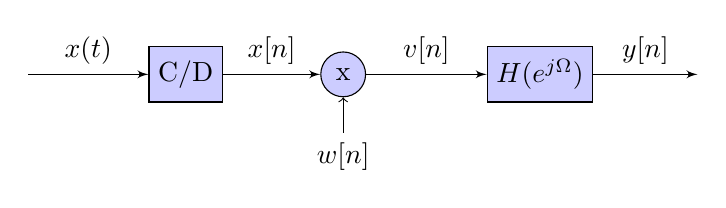
\begin{tikzpicture}[node distance=2.5cm,auto,>=latex']
      \node [int] (a) {C/D};
      \node (b) [left of=a,node distance=2cm, coordinate] {x(t)};
      \node [sum, pin={[init]below:$w[n]$}] (c) [right of=a, node distance=2cm] {x};
      \node [int] (d) [right of=c] {$H(e^{j\Omega})$};
      \node [coordinate] (end) [right of=d, node distance=2cm]{};
      \path[->] (b) edge node {$x(t)$} (a);
      \path[->] (a) edge node {$x[n]$} (c);
      \draw[->] (c) edge node {$v[n]$} (d) ;
      \draw[->] (d) edge node {$y[n]$} (end) ;
  \end{tikzpicture}    
\end{figure}
In real-world DSP systems, we are often converting a continuous time signal into a discrete one via sampling.
Because input is constantly streaming in, we can't process all of it at once, especially for real-time applications.
That is why we instead process blocks of length $L$ at a time. This is accomplished by multiplying by a window function $w[n]$.

All window functions are real, even, and finite. This means they have real and symmetric DTFTs. The most simply window is a box window (a sinc in the frequency domain).
When the signal is multiplied by a window, it amounts to a periodic convolution in the frequency domain
$$V(e^{j\Omega})=\frac{1}{2\pi}\int_{\langle 2\pi \rangle}X(e^{j\Omega})W(e^{j(\Omega-\omega)})d\omega$$
This periodic convolution means our choice of window function has an impact on our ability to resolve frequencies in the frequency domain.
\begin{itemize}
  \item If $W(e^{j\Omega})$ has a wide "main lobe" at the DC frequencies, then the spectrum of $V(e^{j\Omega})$ will be blurred
  \item If $W(e^{j\Omega})$ has large "side lobes" at non DC frequencies, then \textbf{spectral leakage} occurs because larger frequencies start bleeding into lower ones.
\end{itemize}
Another factor which impacts our ability to resolve frequencies in frequency domain is the length of the window. Because an L point DFT samples the DTFT at L points,
taking a larger window will resolve the DTFT better. If we don't want too increase the window length (because doing so would decrease the latency of our system), we can
zero pad after windowing because zero padding has no length on the DFT.
$$\sum_{n=0}^{N-1}{v[n]W_n^k} = \sum_{n=0}^{L-1}{v[n]W_n^k}\qquad \text{ if } \forall L<n<N-1,v[n]=0$$
\subsection{Short Time Fourier Transform (STFT)}
An important part of Spectral Analysis is understanding the frequencies present in a signal. However, by looking at the DFT of a signal $x[n]$, we only get the frequency information
across the entire duration of the signal. Likewise, just by looking at $x[n]$, we get no frequency information and only temporal information. The STFT is a tool to see both at once.
$$X[n, \omega) = \sum_{m=-\infty}^{\infty}x[n+m]w[m]e^{j\omega m}$$
essentially, we slide a window function around x and compute the DTFT at every time point. This creates a map from 1 dimension to 2D. This map is called the spectrogram.
In the STFT, $\omega$ is continuous while $n$ is discrete.
\subsection{Discrete STFT}
Just like the DFT discretizes the DTFT, we can make the STFT purely discrete with the DSTFT.
$$X[r, k] = \sum_{m=0}^{L-1}x[rR+m]w[m]W_N^{km}$$
Just like before, we take our window and slide it around the signal, computing DFTs at every time point.
Our window is of length $L$, $R$ is how much we shift the window around, and $N \ge L$ is the DFT length we are taking.
If $N > L$, then we are essentially computing a zero-padded DFT. This produces a spectrogram which we can display digitally.
To reconstruct the signal from the DSTFT
$$x[rR+m]w_L[m] = \frac{1}{N}\sum_{k=0}^{N-1}X[n, k]W_N^{-km}$$
As long as the window is not 0 and the windows don't overlap, $$x[n] = \frac{x[n-rL]}{w_L[n-rL]}$$
\subsection{Time-Frequency Uncertainty} 
When we compute the spectrogram of a signal, we can think of each coefficient as "tiling" the time-frequency space.
If we consider the normal N point DFT, each DFT coefficient is supported by N points in the time domain. Since the DFT samples the DTFT, it divides the range of $[0, 2\pi]$
into $N$ segments of width $\frac{2\pi}{N}$. Each coefficient represents one of these coefficients, leading to a tiling looking like this (for a 5 point DFT).
\begin{figure}[H]
  \centering
  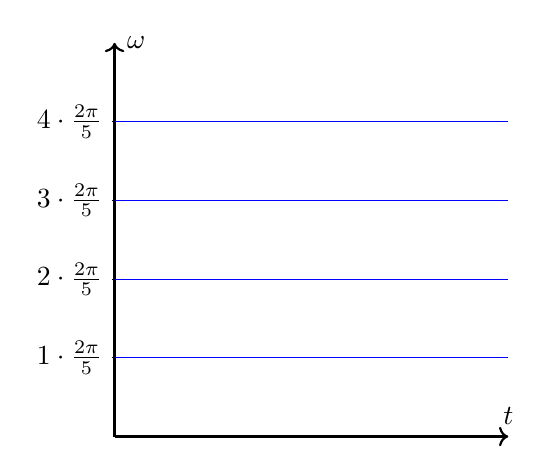
\begin{tikzpicture}
      \draw[thick,->] (0, 0) -- (5,0);
      \draw[thick,->] (0,0) -- (0,5);
      \draw (5 cm,1pt) node[anchor=south] {$t$};
      \draw (1pt,5cm) node[anchor=west] {$\omega$};
      \foreach \y in {1, 2, 3, 4}
          \draw (1pt,\y cm) -- (-1pt,\y cm) node[anchor=east] {$\y\cdot \frac{2\pi}{5}$};
      \draw[scale=1,domain=0:5,smooth,variable=\x,blue] plot ({\x},{1});
      \draw[scale=1,domain=0:5,smooth,variable=\x,blue] plot ({\x},{2});
      \draw[scale=1,domain=0:5,smooth,variable=\x,blue] plot ({\x},{3});
      \draw[scale=1,domain=0:5,smooth,variable=\x,blue] plot ({\x},{4});
  \end{tikzpicture}  
\end{figure}
Thinking about the DSTFT, each coefficient is computed using $L$ points of the original signal. Each coefficient
still represents intervals of $\frac{2\pi}{N}$ in the frequency axis. This leads to a tiling which looks like this.
\begin{figure}[H]
  \centering
  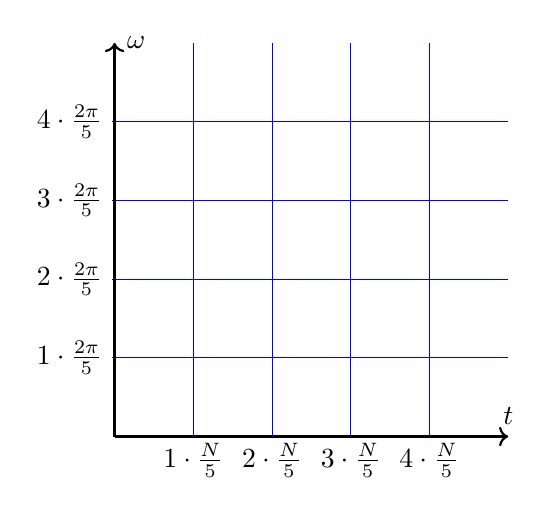
\begin{tikzpicture}
      \draw[thick,->] (0, 0) -- (5,0);
      \draw[thick,->] (0,0) -- (0,5);
      \draw (5 cm,1pt) node[anchor=south] {$t$};
      \draw (1pt,5cm) node[anchor=west] {$\omega$};
      \foreach \y in {1, 2, 3, 4} {
          \draw (1pt,\y cm) -- (-1pt,\y cm) node[anchor=east] {$\y\cdot \frac{2\pi}{5}$};
          \draw[scale=1,domain=0:5,smooth,variable=\x,blue] plot ({\x},{\y});
      }
      \foreach \x in {1, 2, 3, 4} {
          \draw (\x cm, 1pt) -- (\x cm, 1pt) node[anchor=north] {$\x\cdot \frac{N}{5}$};
          \draw[scale=1,domain=0:5,smooth,variable=\y,blue] plot ({\x},{\y});
      }
  \end{tikzpicture}  
\end{figure}
What these tilings show us is that because we have discretized time and frequency,
there is some uncertainty regarding which times and frequencies each coefficient represents.

We can formalize this idea by considering a general transform. All transforms are really an inner product with a set of basis functions
$$T_x(\gamma) = \langle x(t), \phi_\gamma(t) \rangle=\int_{-\infty}^{\infty}x(t)\phi_\gamma^\star(t)dt$$
For each particular $\gamma$, that $T_x(\gamma)$ is the projection of our signal onto the basis vector $\phi_\gamma(t)$. We can use Parseval's relationship
to see that
\begin{align*}
  T_x(\gamma) &= \langle x(t), \phi_\gamma(t) \rangle =\int_{-\infty}^{\infty}x(t)\phi_\gamma^\star(t)dt \\
  &= \frac{1}{2\pi}\int_{-\infty}^{\infty}X(j\Omega)\Phi_\gamma^\star(j\Omega)d\Omega \\
  &= \langle X(j\Omega), \frac{1}{2\pi}\Phi_\lambda(j\Omega)\rangle
\end{align*}
This means that we can equivalently think of projecting the spectrum of our signal onto the spectrum of our basis function. Remember that projection essentially asks "How much of a signal can be explained by the basis".
We can formalize this by looking at the signal in a statistical sense and treat it as a probability distribution.
\begin{align*}
  m_t &= \int_{-\infty}^{\infty}t|\psi(t)|^2dt &\qquad m_\Omega &= \int_{-\infty}^{\infty}\Omega\frac{1}{2\pi}|\Psi(j\Omega)|^2d\Omega\\
  \sigma_t^2 &= \int_{-\infty}^{\infty}(t-m_t)^2|\psi(t)|^2dt &\qquad \sigma^2_\Omega &= \int_{-\infty}^{\infty}(\Omega-m_\Omega)^2\frac{1}{2\pi}|\Psi(j\Omega)|^2d\Omega\\
\end{align*}
$m_t$ and $m_\Omega$ are the means of the signal and the spectrum. $\sigma_t^2$ and $\sigma_\Omega^2$ are the variances. Together, they localize where our signal "lives" in the time-frequency spectrum.
The uncertainty principle says
$$\sigma_t\sigma_w \ge \frac{1}{2}$$
This means there is nothing we can do to get completely accurate time resolution and frequency resolution, and any decisions we make will
lead to a tradeoff between them.
\subsection{Wavelets}
While the STFT gives us a better picture of a signal than a full-length DFT, one of its shortcomings is that each coefficient is supported by the same amount of time and frequency. Low frequencies don't change as
much as high frequencies do, so a lower frequency needs to be resolved with more time support whereas a fast signal would requires less time support to resolve properly.
The Wavelet transform takes this idea and tiles the Time-Frequency spectrum with different time and frequency supports (essentially making all of the boxes different sizes) by using a scaled bandpass filter $\Psi(t)$ as its kernel.
$$\int_{-\infty}^{\infty}|\Psi(t)|^2dt=1 \qquad \int_{-\infty}^{\infty}\Psi(t)dt = 0$$
This kernel is called the mother wavelet. The continuous wavelet transform then becomes.
$$Wf(u, s) = \int_{-\infty}^{\infty}f(t)\frac{1}{\sqrt{s}}\Psi^\star\left(\frac{t-u}{s}\right)dt$$
We need an infinite number of functins to fully represent all frequencies properly, but at a certain level, we don't care about our ability to resolve them better, so we stop scaling and
use a low frequency function $\Phi(t)$ to "plug" the remaining bandwidth. this is called the "father" wavelet.
\subsubsection{Discrete Wavelet Transform}
In discrete time, the wavelet transform becomes
$$d_{s,u}=\sum_{n=0}^{N-1}x[n]\Psi_{s,u}[n] \qquad a_{s,u}=\sum_{n=0}^{N-1}x[n]\Phi_{s,u}[n]$$
The $d$ coefficients are the detailed coefficients and are computed using the mother wavelet. The capture higher frequency information.
The $a$ coefficients are the approximate coefficients computed using the father wavelet. They represent lower frequency information.
The time frequency tiling for the DWT looks something like this.
\begin{figure}[H]
  \centering
  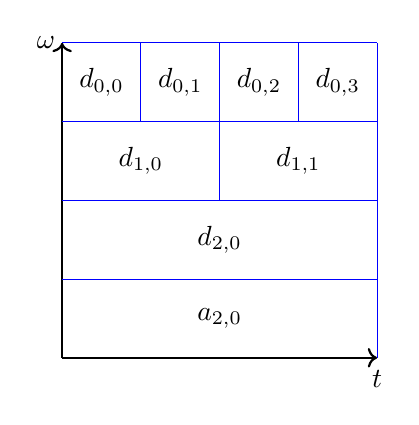
\begin{tikzpicture}
      \draw[thick,->] (0, 0) -- (4,0);
      \draw[thick,->] (0,0) -- (0,4);
      \draw (4 cm,-1pt) node[anchor=north] {$t$};
      \draw (1pt,4cm) node[anchor=east] {$\omega$};
      \foreach \y in {1, 2, 3, 4} {
          \draw[scale=1,domain=0:4,smooth,variable=\x,blue] plot ({\x},{\y});
      }
      \foreach \x in {1, 2, 3} {
          \draw[scale=1,domain=3:4,smooth,variable=\y,blue] plot ({\x},{\y});
      }
      \draw[scale=1,domain=0:4,smooth,variable=\y,blue] plot ({4},{\y});
      \draw[scale=1,domain=2:3,smooth,variable=\y,blue] plot ({2},{\y});
      \draw (0.5cm,3.5cm) node[] {$d_{0,0}$};
      \draw (1.5cm,3.5cm) node[] {$d_{0,1}$};
      \draw (2.5cm,3.5cm) node[] {$d_{0,2}$};
      \draw (3.5cm,3.5cm) node[] {$d_{0,3}$};
      \draw (1cm,2.5cm) node[] {$d_{1,0}$};
      \draw (3cm,2.5cm) node[] {$d_{1,1}$};
      \draw (2cm,1.5cm) node[] {$d_{2,0}$};
      \draw (2cm,0.5cm) node[] {$a_{2,0}$};
  \end{tikzpicture}  
\end{figure}
Notice how each Wavelet coefficient is supported by a different amount of time and frequency.
We can choose different mother and father wavelets to describe our signals. For example, the Haar wavelet
does very well with piecewise constant signals.
\end{document}